\chapter{Introduction \todomatthew{almost finished}}

\section{Motivation}

The natural world is rich in visual texture. While a precise definition of 
texture remains to be found, most research consider it as visual patterns that 
exhibit local spatial variations while maintaining global homogeneity \todomatthew{figure of a texture}. Textures 
can be static or dynamic: static textures exist in two-dimensional (2D) image space 
(\eg, grass and water) while dynamic textures extend the notion across time (\eg, 
fluttering grass and wavy water). As a result, local spatial variations and 
global homogeneity extend across space \emph{and} time. These temporal patterns 
have previously been studied under a variety of names, including turbulent-flow 
motion \cite{heeger1986}, temporal textures \cite{nelson1992}, time-varying 
textures \cite{bar-joseph2001}, dynamic textures \cite{doretto2003}, textured 
motion \cite{wang2003} and spacetime textures \cite{derpanis2012spacetime}.
In this thesis, the term ``dynamic texture'' is adopted. \todomatthew{1 sentence for each reference with a short description of the work and the context. }

Both static and dynamic texture cues play important roles in our perception of 
surfaces. Understanding and characterizing these patterns has long been a problem 
of interest in human perception, computer vision, and computer graphics. In 
computer vision, studying the underlying statistics of textures allows us to gain 
insight as to how these complex structures can be interpreted and how we may be 
able to leverage this knowledge to inform certain vision-related tasks. Examples 
of such tasks include shape from texture \cite{gibson1950perception}, texture 
synthesis \cite{heeger1995pyramid}, and more recently, image style transfer 
\cite{gatys2016image}.

Shape from texture involves recovering the
three-dimensional (3D) shape of an object from a 2D image by using texture as a 
cue. Gibson \cite{gibson1950perception} proposed the \emph{texture gradient} as 
the primary basis of surface perception by humans. He revealed that neighbouring areas on a textured surface are perceived differently only due to differences
in surface orientation and distance from the observer.

Texture synthesis \todomatthew{perhaps include a figure of texture synthesis} is the process of algorithmically constructing a texture that
matches or extends a given source texture by taking advantage of its structural 
content. Heeger and Bergen \cite{heeger1995pyramid} took advantage of the fact 
that two textures are often difficult to discriminate when they produce a similar 
distribution of responses from a bank of linear filters. They used a combination 
of Laplacian and steerable pyramids to deconstruct a given texture and 
synthesized a new texture by matching the distributions of responses from each
pyramid level. Image style transfer \todomatthew{include style transfer figure} is a recent extension of texture synthesis where the goal is to 
synthesize a texture from a source image while constraining the process in order 
to preserve the semantic content of another image. This can be considered as a 
texture transfer problem \todomatthew{cite texture transfer papers}. Gatys \etal \cite{gatys2016image} demonstrated 
impressive results by using a convolutional network (ConvNet) instead of a linear 
bank of filters to model the non-linear spatial statistics of a given texture and semantic content of a given image. The focus of this work is on the synthesis of dynamic texture 
samples based on a single exemplar through the use of ConvNets. \todomatthew{discuss the previous use of purely filter driven characterizations of textures and the current use of CNNs.}

\section{Outline of thesis}

Many common dynamic textures are naturally described by the ensemble of 
appearance and dynamics (\ie, spatial and temporal pattern variation) of their 
constituent elements. In this work, a factored analysis of dynamic 
textures in terms of their appearance and dynamics is proposed.
This factorization is then used to enable dynamic texture synthesis
which, based on example dynamic texture inputs, will generate a novel dynamic
texture instance.
It shall also enable a novel form of style transfer where the 
target appearance and dynamics can be taken from different sources---termed \emph{dynamics style transfer}.
An overview of dynamic texture synthesis and dynamics style transfer
is shown in Fig.\ \ref{fig:teaser}.

\begin{figure}[t]
\begin{center}
	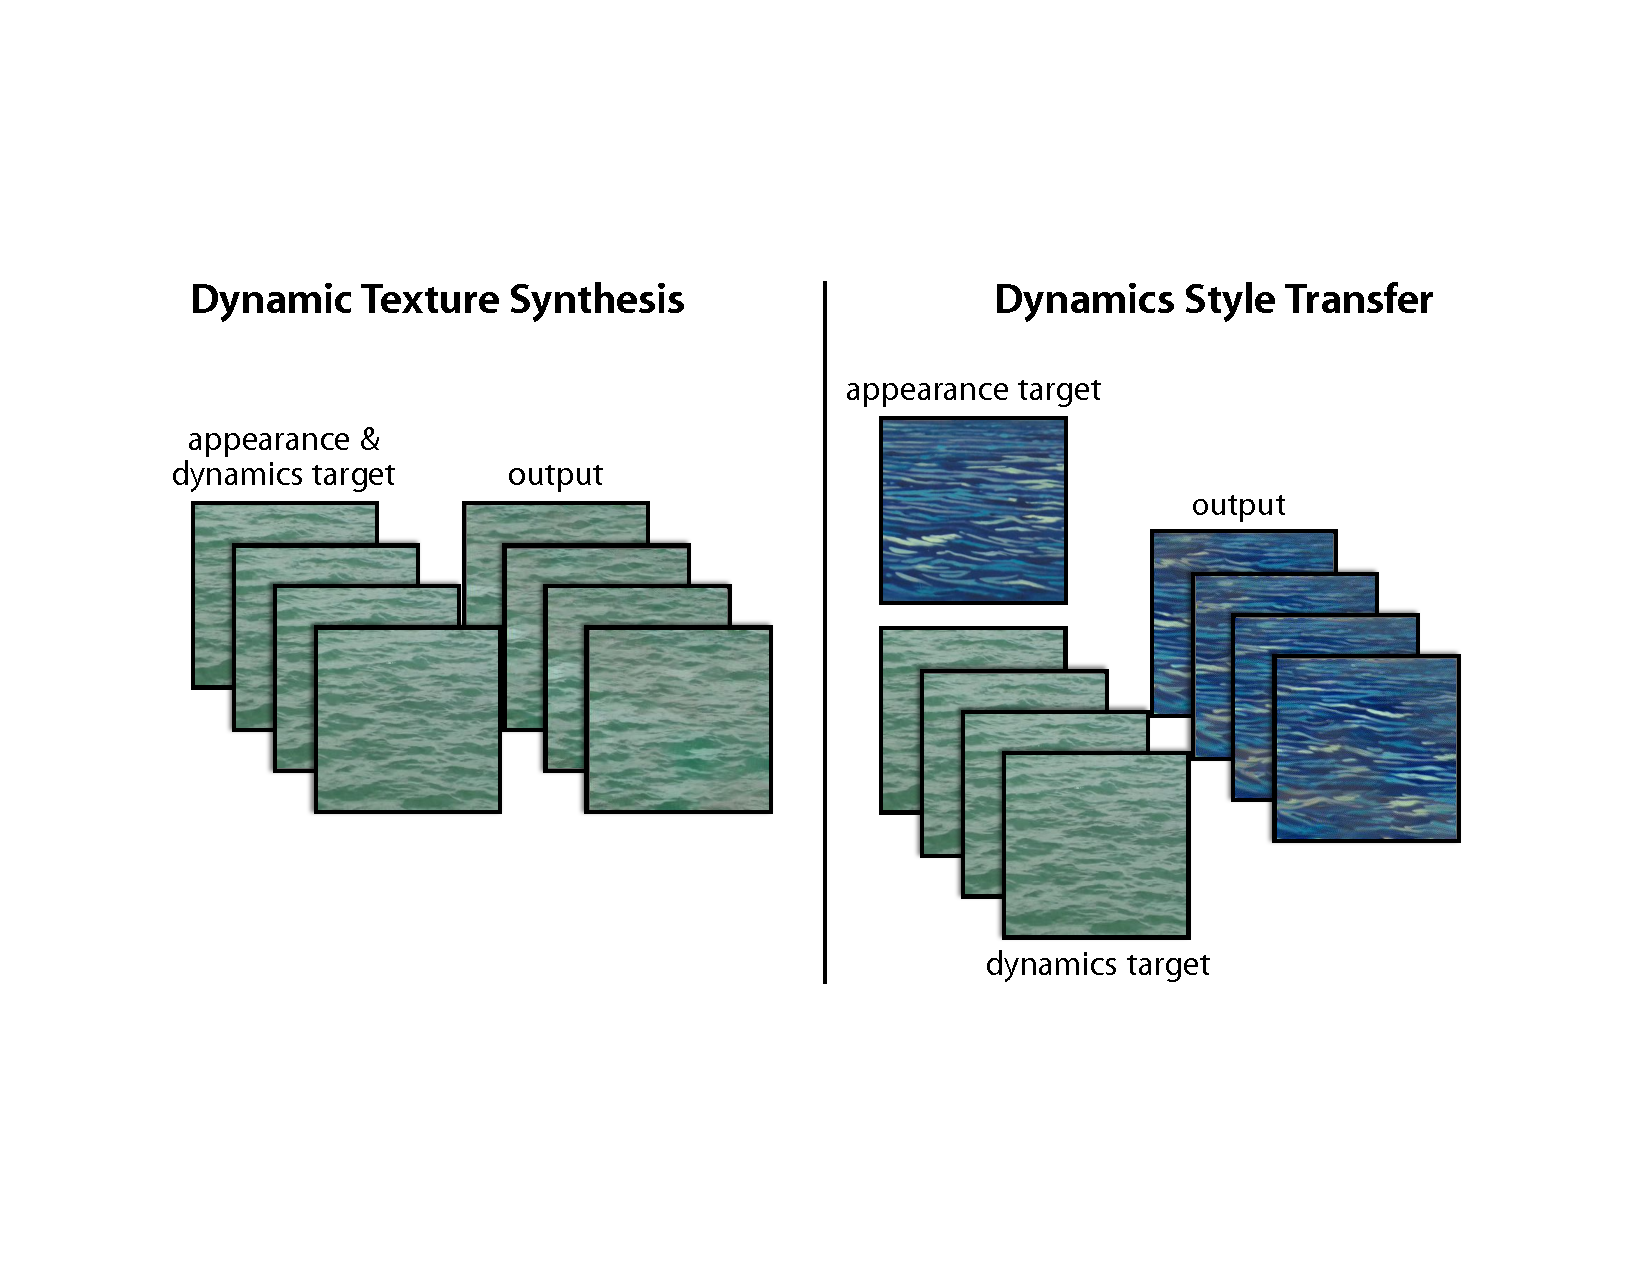
\epsfig{file=teaser.pdf, width = 0.8\textwidth}\\
	\caption[Dynamic texture synthesis.]{Dynamic texture synthesis. (left) Given an input dynamic texture as the target, the two-stream model synthesizes a novel dynamic texture that preserves the target's appearance and dynamics characteristics. (right) The two-stream approach enables synthesis that combines the texture appearance from one target with the dynamics from another, resulting in a composition of the two.}
	\vspace{-0.65cm}
	\label{fig:teaser}
\end{center}
\end{figure}

The proposed model is constructed from two ConvNets: an appearance stream and a dynamics stream,
which have been pre-trained for object recognition
and optical flow prediction, respectively.
Similar to previous work on spatial textures
\cite{gatys2015,heeger1995pyramid,portilla2000parametric}, an input dynamic texture is summarized in terms of a set of
spatiotemporal statistics of filter outputs from each stream.
The appearance stream models the per-frame appearance of
the input texture, while the dynamics stream models its
temporal dynamics.
The synthesis process consists of optimizing a randomly initialized noise pattern such that its spatiotemporal statistics from
each stream match those of the input texture.
The architecture is inspired by insights from human perception and 
neuroscience.
In particular, psychophysical studies \cite{cutting1982} show that
humans are able to perceive the structure of a dynamic texture even
in the absence of appearance cues, suggesting that the two streams
are effectively independent.
Similarly, the two-stream hypothesis \cite{goodale1992} models the 
human visual cortex in terms of two pathways, the ventral stream
(involved with object recognition) and the
dorsal stream (involved with motion processing).

In this thesis, the two-stream analysis of
dynamic textures is applied to texture synthesis.
A range of dynamic textures are considered and it is demonstrated that the 
proposed approach generates novel, high quality samples that match
both the frame-wise appearance and temporal evolution of an input
example.
Further, as stated previously, the factorization of appearance and dynamics enables a 
novel form of style transfer, where the dynamics of one texture are 
combined with the appearance of a different one,
\cf\ \cite{gatys2016image}.
This can even be done using a single image as an appearance
target, which allows static images to be animated.
Finally, the perceived realism of the generated textures is validated
through an extensive user study.

\section{Contributions}

The contributions of this work span both theory and application. First,
theoretical insight into the characterization of dynamic textures is provided by 
building a novel factored representation of both appearance and dynamics. Second, 
for the representation of dynamics, a novel ConvNet is constructed and trained for 
optical flow prediction. Third, through a qualitative evaluation, it is shown that the two-stream representation is 
effective in generating visually compelling, novel instances of a wide range of 
dynamic textures. Fourth, a novel form of style transfer is demonstrated, 
where the dynamics of a dynamic texture can be mixed with the spatial appearance 
of a different (static or dynamic) texture. This is enabled by the proposed factored 
representation. Finally, a quantitative evaluation on the limitations of the method is performed through 
the inclusion of a broad range of textures and an extensive user study. This analysis will show which 
sequences work better than others and why. This may point to future work to 
address limitations of the proposed model. In terms of specific applications, 
there are many in the creative-industry including, but not limited to, computer-
generated imagery, digital painting, and image editing. More broadly, the ability 
to animate static imagery via dynamics style transfer can meaningfully contribute 
to the emerging artistic medium of computer-generated art.